\chapter{প্রোগ্রামিং সহ বিভিন্ন ব্যবহৃত লেখার নমুনা}

\section{তালিকা}

নিম্নোক্ত উপায়ে তালিকা করা যেতে পারে।
\begin{itemize}
\item uva.onlinejudge.org প্রোগ্রামিং প্রতিযোগিতার জন্য সবচেয়ে জনপ্রিয় ওয়েবসাইট। এখানে প্রায়ই ৫ ঘণ্টার প্রতিযোগিতা হয়ে থাকে বিশেষ করে অক্টোবর থেকে ডিসেম্বর এই সময়ে। এছাড়াও এখানে আছে ৪০০০ এরও বেশি প্র্যাকটিস প্রবলেম। 
\item icpcarchive.ecs.baylor.edu এটা uva ওয়েবসাইটের ভাই। এখানে 1988 সাল থেকে শুরু করে আজ পর্যন্ত হয়ে আসা বহু ICPC Regional Programming Contest এবং ACM ICPC World Finals এর প্রবলেমসমূহ আছে।
\item acm.sgu.ru রাশিয়ান প্রোগ্রামিং সাইট। এখানে তুলনামূলকভাবে অনেক কম প্রবলেম আছে, কিন্তু একেকটা সমস্যা সমাধান করতে মাথার ঘাম পায়ে পড়ে! যদি কেউ এখানের সবগুলো সমস্যা সমাধান করে তাহলে আমার মনে হয় না সে কোথাও সহজে আটকাবে।
\item acm.timus.ru আরও একটি রাশিয়ান সাইট। এখানে প্রবলেমগুলো বেশ কিছু ক্যাটাগরিতে ভাগ করা আছে। তোমরা যারা নতুন নতুন প্রোগ্রামিং শুরু করেছ তারা এই সাইটের Beginners Problem সেকশনের 20টি সমস্যা সমাধান করে দেখতে পার। এগুলো সমাধান করতে কোনো অ্যালগরিদম বা ডেটা স্ট্রাকচারের দরকার হয় না, শুধু প্রোগ্রামিং ল্যাঙ্গুয়েজ জানলেই চলে। এখানের সমস্যাগুলোও বেশ কঠিন হয়, হাজার হোক রাশিয়ান প্রবলেম বলে কথা! একবার আমাদের দেশের এক world finalist এর সঙ্গে কথা হচ্ছিল, সে গর্ব করে বলছিল যে সে একবার timus এর কোন এক প্রতিযোগিতার সমস্যা সমাধান করেছিল। আমি বললাম- হ্যাঁ timus এর প্রতিযোগিতার সমস্যাগুলো বেশ কঠিন হয়, কনটেস্ট সময়ে একটা করতেই খবর খারাপ হয়। তখন সে বলে যে সে আসলে কনটেস্ট এর তিন চারদিন পর সমাধান করেছিল। মানে এই সমস্যাগুলি এতোই কঠিন যে সেটা আসলে তিন চার দিন পর সমাধান করতে পারলেও বেশ বড় ব্যাপার বলা যায়! তার মানে কি তুমি কঠিন বলে এসব সাইট এর সমস্যা সমাধান করবে না? এসব সাইটে কনটেস্ট করবে না? মোটেও না। তুমি যদি কঠিন কঠিন সমস্যা সমাধান না কর তোমার উন্নতি হবে না! হয়তো তুমি ICPC তে champion হয়ে world finals এ যাবে কিন্তু এরপর দেখবে আর চাইনিজ, পোলিস বা রাশিয়ানদের সাথে পেরে উঠছ না।
\item {\bnbf কিছু চাইনিজ অনলাইন জাজ:} বেশ কিছু চাইনিজ OJ আছে। acm.pku.edu.cn, acm.zju.edu.cn, acm.tju.edu.cn এই তিনটি প্রধান বলতে পার। pku সাইটে আগে মাসিক কনটেস্ট হতো এবং তার অ্যানালাইসিস পাবলিশ করা হতো। এখনো pku এবং zju সাইটে কনটেস্ট হয়ে থাকে। tju ওয়েবসাইটেও অনেক প্রবলেম আছে, তবে মূলত এখানে প্র্যাকটিস কনটেস্ট আয়োজন করা হয়ে থাকে। এসব সাইটে আসলে সহজ কঠিন সব ধরনের সমস্যা আছে। তবে আমার মনে হয়েছে চাইনিজ কঠিন সমস্যাগুলো রাশিয়ান কঠিন সমস্যাগুলোর থেকেও কঠিন হয়! একবার এক চাইনিজ প্রবলেমসেটার ঘোষণা দিয়েছিল যে, যদি কেউ তার অমুক সমস্যা পরবর্তী এক বছরে সমাধান করে তাহলে তাকে সে পুরস্কার দেবে। আমি ঠিক জানি না কেউ সমাধান করেছিল কিনা। এছাড়াও Rujia Liu এর কিছু সমস্যা তুমি uva তে খুঁজে পাবে (তার নাম দিয়ে আলাদা সেকশনই আছে uva তে), যার প্রতিটি সমস্যাই খুবই শিক্ষণীয়। Rujia Liu একসময় চীনের IOI দলকে প্রশিক্ষণ দিতেন, নিজেও ACM World finals এ মেডেল জিতেছিলেন।
\end{itemize}

\section{কম্পিউটার প্রোগ্রাম}
এভাবে করে কম্পিউটার প্রোগ্রামের কোড দেওয়া যেতে পারে (কোড ~\ref{code:simple-code})।  ইনলাইনে ম্যাথমোডে সংখ্যা ব্যবহার করা যায়, যেমন: $6 + 2 = 8$.

\lstinputlisting[label={code:simple-code},caption={simple code.cpp}]{code/chapter_2/simple_code.cpp}


\section{ডেফিনেশন লিস্ট}
কিন্তু তোমরা ভাবতে পার যে এই একটা যোগ করতেই এত বড় কোড লিখতে হয়? আসলে খুব শীঘ্রই বুঝতে পারবে যে খুব ছোট কোড দিয়ে কীভাবে অনেক বড় বড় কাজ করে ফেলা যায়। কেবল তো শুরু! যাই হোক, বেশি দূরে যাওয়ার আগে সংক্ষেপে দেখে নেই প্রতিটা লাইনের মানে:
\begin{description}
\item[Line 1] stdio.h নামের হেডার (header) ফাইল কে ইনক্লুড (include) করা হয়েছে। বিভিন্ন ধরনের হেডার ফাইল আছে। এই ফাইলটির কাজ হলো ইনপুট আউটপুটের কাজ করা। stdio এর পূর্ণ অর্থ হলো স্ট্যান্ডার্ড ইনপুট আউটপুট (standard input output).
\item[Line 2] ফাঁকা লাইন। আমরা কোডের সৌন্দর্যের জন্য এরকম ফাঁকা লাইন বা স্পেস (space) বা ট্যাব (tab) দিয়ে থাকি। এতে করে পরবর্তীতে কোড বুঝতে সুবিধা হয়।
\item[Line 3] এখান থেকে মেইন ফাংশন (main function) শুরু হয়েছে। যখন তোমার কোড রান (run) করবে তখন এই ফাংশন থেকেই কাজ শুরু হয়। আর এই ফাংশন একটি ইন্টিজার (integer) ডেটা রিটার্ন (return) করে।
\item[Line 5] এখানে দুটি সংখ্যার যোগফল প্রিন্ট করা হচ্ছে। তুমি যদি একই সঙ্গে যোগফল এবং বিয়োগফল প্রিন্ট করতে চাও তাহলে printf("\%d \%d\textbackslash n", 6 + 2, 6 - 2) এভাবে লিখতে পার। বুঝতেই পারছ যে যখন কোনো একটি সংখ্যা প্রিন্ট করতে চাও তখন তোমাকে \%d ব্যবহার করতে হবে। এখন তুমি নিজে একটা কাজ কর তা হলো এই লাইনকে পরিবর্তন করে লেখ printf("Summation is \%d, Difference is \%d\textbackslash n", 6 + 2, 6 - 2). কী প্রিন্ট হয় দেখতো। আশা করি বুঝতে পারছ কীভাবে তোমার পছন্দ মতো কথাবার্তা এবং সেই সাথে তোমার হিসাবনিকাশের ফলাফল তুমি প্রিন্ট করতে পারবে। আরেকটি কথা, এই printf ফাংশনটি আউটপুটের কাজ করছে। আর এটি ব্যবহারের জন্যই আমরা প্রথম লাইনে stdio.h হেডার ফাইলটি ইনক্লুড করেছি। আমাদের আরও অনেক হেডার ফাইল আছে, আমরা ধীরে ধীরে সেসব সম্পর্কে জানব।
\item[Line 6] মেইন ফাংশনটি $0$ সংখ্যা রিটার্ন করবে। আমরা সবসময় $0$ রিটার্ন করব। অন্য কিছু রিটার্ন করলে অপারেটিং সিস্টেম (operating system) মনে করে যে তোমার প্রোগ্রামটি ঠিক মত শেষ হয় নাই।
\end{description}


\section{ইনলাইন লিস্ট}
\begin{inparaitem}
\item \href{http://acm.timus.ru/problem.aspx?space=1&num=1000}{Timus 1000}
\item \href{http://acm.timus.ru/problem.aspx?space=1&num=1264}{Timus 1264}
\item \href{http://acm.timus.ru/problem.aspx?space=1&num=1293}{Timus 1293}
\item \href{http://acm.timus.ru/problem.aspx?space=1&num=1409}{Timus 1409}
\end{inparaitem}

\section{টেবিল}

আমরা এখন পর্যন্ত একটাই হেডার ফাইল দেখেছি- stdio.h. আরও একটি হেডার ফাইল দেখা যাক, এটা হলো math.h হেডার ফাইল। নাম দেখেই বোঝা যাচ্ছে এখানে গণিত সংক্রান্ত কিছু ফাংশন দেওয়া আছে। আমাদের ক্যালকুলেটরে যেমন অনেক ফাংশন আছে (যেমন sin, cos, tan, square root, square, cube ইত্যাদি) ঠিক তেমনি এই math.h হেডার ফাইলে এ ধরনের বেশ কিছু ফাংশন আছে। টেবিল \ref{tab:mathh} তে math.h এর কিছু গুরুত্বপূর্ণ ফাংশন দেওয়া হলো। 

\begin{table}[!hbt]
	\caption{math.h এর কিছু ফাংশনের তালিকা \label{tab:mathh}}
	\begin{center}\begin{footnotesize}
	\begin{tabular}{|l|p{8cm}|}
		\hline
		sqrt(x) & এটা $x$ এর বর্গমূল (square root) নির্ণয় করে। $x$ কে অবশ্যই অঋণাত্মক হতে হবে। না হলে Run Time Error (RTE) হবে। \\\hline
		fabs(x) & এটা $x$ এর পরম মান (absolute value) নির্ণয় করে। \\\hline
		sin(x), cos(x), tan(x) & $x$ এর $\sin, \cos, \tan$ নির্ণয় করে থাকে। এখানে $x$ কে রেডিয়ান (radian) এককে দিতে হবে। \\\hline
		asin(x), acos(x), atan(x) & $x$ এর $\sin^{-1}, \cos^{-1}, \tan^{-1}$ নির্ণয় করে থাকে। এখানে $\sin^{-1}$ এবং $\cos^{-1}$ এর ক্ষেত্রে $x$ কে অবশ্যই $[-1, 1]$ সীমার মধ্যে হতে হয় এবং রিটার্ন মানটি রেডিয়ান এককে থাকে। \\\hline
		atan2(y, x) & উপরের asin, acos এর মতোই। তবে যেহেতু $\Delta y = 1, \Delta x = 0$ হলে $\tan^{-1}$ এর মান $atan$ ফাংশন দিয়ে বের করা যায় না ($atan$ এ তোমাকে $\frac{\Delta y}{\Delta x}$ দিতে হবে আর তা দিতে গেলে division by zero হয়ে যাবে), সেহেতু সেক্ষেত্রে আমরা atan2 ব্যবহার করতে পারি।\\\hline
		pow(x, y) & এটি $x^y$ নির্ণয় করে থাকে।\\\hline
		exp(x) & এটি $e^x$ নির্ণয় করে।\\\hline
		log(x), log10(x) & এখানে log হলো স্বাভাবিক  লগারিদম(natural logarithm)   আর log10 হলো 10 ভিত্তিক লগারিদম। \\\hline
		floor(x), ceil(x) & যথাক্রমে floor এবং ceiling দেয়।\\\hline
	\end{tabular}
	\end{footnotesize}\end{center}
\end{table}


\section{জেপেগ (jpeg) ছবি}
$n$ ইনপুটের জন্য চিত্র \ref{fig:pyramid} এর পিরামিডগুলো প্রিন্ট করার প্রোগ্রাম লিখ। না তোমাকে সবগুলি পিরামিড একত্রে প্রিন্ট করতে হবে না। আলাদা আলাদা করে প্রিন্ট করলেই চলবে। 
\begin{figure}[ht!]
	\centering
	\includegraphics[width=90mm]{image/chapter_2/pyramid.jpg}
	\caption{কিছু পিরামিড $n = 3$ এর জন্য}
	\label{fig:pyramid}
\end{figure}

\section{সমীকরন}

\begin{align*}
& 1 + (1 + 2) + (1 + 2 + 3) + \ldots + (1 + 2 + \ldots + n) \\
&= \sum_{i = 1}^{n} {\sum_{j = 1}^{i} {j}} \\
&= \sum_{i = 1}^{n} { \frac{i^2 + i}{2} } \\
&= \frac{1}{2} \left( \sum_{i = 1}^{n} {i^2} + \sum_{i = 1}^{n} {i} \right) \\
&= \frac{1}{2} \left( \frac{n(n + 1)(2n + 1)}{6} + \frac{n^2 + n}{2} \right)
\end{align*}

বিগ-ও-নোটেশনের জন্য কাস্টম স্টাইলিং যেমন: আমরা লুপ ব্যবহার না করে শুধু কিছু যোগ আর গুণ করেই করে ফেলতে পারি, একে বলা হয় \BigO{1} অ্যালগরিদম।

তোমরা আশা করি ফিবোনাচি সংখ্যার(Fibonacci Number) কথা শুনেছ। যারা শুনো নাই তাদের জন্য বলি, $n$তম ফিবোনাচি সংখ্যাকে $F_n$ দিয়ে প্রকাশ করা হয়। এর মান:

\[
	F_n =
	\begin{cases}
		0  & n = 0 \\
		1 & n = 1 \\
		F_{n - 1} + F_{n - 2} & n \geq 2
	\end{cases}
\]

\section{কোটেশন}

{\fontfamily{uncl}\selectfont
\begin{quotation}
I learned a second lesson in the 60s, when I taught a course on programming to sophomores and discovered to my surprise that 10\% of my audience had the greatest difficulty in coping with the concept of recursive procedures. I was surprised because I knew that the concept of recursion was not difficult. Walking with my five-year old son through Eindhover, he suddenly said ``Dad, not every boat has a life-boat, has it?" ``How come?" I said. ``Well, the life-boat could have a smaller life-boat, but then that would be without one." It turned out.
\end{quotation}
}

\section{ম্যাট্রিক্স}

ম্যাট্রিক্স ব্যবহার করে আমরা লিখতে পারি:

\begin{align*}
\begin{bmatrix} F _2 \\ F_1 \end{bmatrix} &= \begin{bmatrix} 1 & 1 \\ 1 & 0 \end{bmatrix} \begin{bmatrix} F_1 \\ F_0 \end{bmatrix} \\
\begin{bmatrix} F _3 \\ F_2 \end{bmatrix} &= \begin{bmatrix} 1 & 1 \\ 1 & 0 \end{bmatrix} \begin{bmatrix} F_2 \\ F_1 \end{bmatrix} \\
&= \begin{bmatrix} 1 & 1 \\ 1 & 0 \end{bmatrix} \begin{bmatrix} 1 & 1 \\ 1 & 0 \end{bmatrix} \begin{bmatrix} F_1 \\ F_0 \end{bmatrix} \\
&= \begin{bmatrix} 1 & 1 \\ 1 & 0 \end{bmatrix}^2 \begin{bmatrix} F_1 \\ F_0 \end{bmatrix} \\
\end{align*}

একইভাবে,
\begin{align*}
\begin{bmatrix} F _4 \\ F_3 \end{bmatrix} = \begin{bmatrix} 1 & 1 \\ 1 & 0 \end{bmatrix}^3 \begin{bmatrix} F_1 \\ F_0 \end{bmatrix} \\
\end{align*}

সুতরাং আমরা লিখতে পারি,
\begin{align*}
\begin{bmatrix} F _n \\ F_{n-1} \end{bmatrix} = \begin{bmatrix} 1 & 1 \\ 1 & 0 \end{bmatrix}^{n-1} \begin{bmatrix} F_{1} \\ F_{0} \end{bmatrix} \\
\end{align*}


\section{একাধিক পৃষ্ঠায় বিস্তৃত টেবিল}


\begin{center}
\begin{longtable}{|c|c|c|}
\caption{গাউসের এলিমিনেশনের উদাহরণ\label{tab:gaussbig}} \\

\hline
\multicolumn{1}{|c|}{\textbf{Operation}} & \multicolumn{1}{c|}{\textbf{Equations}} & \multicolumn{1}{c|}{\textbf{Matrix}}\\
\hline 
\endfirsthead

\multicolumn{3}{c}
{{\bfseries \tablename\ \thetable{} -- পূর্বের পাতা থেকে}} \\
\hline \multicolumn{1}{|c|}{\textbf{Operation}} &
\multicolumn{1}{c|}{\textbf{Equations}} &
\multicolumn{1}{c|}{\textbf{Matrix}} \\ \hline 
\endhead

\multicolumn{3}{|r|}{{পরের পাতায় চলমান}} \\ \hline
\endfoot

\hline
\endlastfoot
শুরু & $\begin{array}{c} 2x -y +3z = 15 \\ 4x -2y +2z = 42 \\ x +y -z = 9 \end{array}$ & $\left[\begin{array}{ccc} 2 & -1 & 3 \\ 4 & -2 & 2 \\ 1 & 1 & -1 \end{array}\right] \left[ \begin{array}{c} x \\ y \\ z \end{array}\right] = \left[ \begin{array}{c} 15 \\ 42 \\ 9 \end{array}\right]$\\[20pt] 
\hline
$\frac{E_1}{2}$ & $\begin{array}{c} x -\frac{1}{2}y +\frac{3}{2}z = \frac{15}{2} \\ 4x -2y +2z = 42 \\ x +y -z = 9 \end{array}$ & $\left[\begin{array}{ccc} 1 & -\frac{1}{2} & \frac{3}{2} \\ 4 & -2 & 2 \\ 1 & 1 & -1 \end{array}\right] \left[ \begin{array}{c} x \\ y \\ z \end{array}\right] = \left[ \begin{array}{c} \frac{15}{2} \\ 42 \\ 9 \end{array}\right]$\\[20pt] 
\hline
$E_2 - 4E_1$ & $\begin{array}{c} x -\frac{1}{2}y +\frac{3}{2}z = \frac{15}{2} \\ -4z = 12 \\ x +y -z = 9 \end{array}$ & $\left[\begin{array}{ccc} 1 & -\frac{1}{2} & \frac{3}{2} \\ 0 & 0 & -4 \\ 1 & 1 & -1 \end{array}\right] \left[ \begin{array}{c} x \\ y \\ z \end{array}\right] = \left[ \begin{array}{c} \frac{15}{2} \\ 12 \\ 9 \end{array}\right]$\\[20pt] 
\hline
$E_3 - E_1$ & $\begin{array}{c} x -\frac{1}{2}y +\frac{3}{2}z = \frac{15}{2} \\ -4z = 12 \\ +\frac{3}{2}y -\frac{5}{2}z = \frac{3}{2} \end{array}$ & $\left[\begin{array}{ccc} 1 & -\frac{1}{2} & \frac{3}{2} \\ 0 & 0 & -4 \\ 0 & \frac{3}{2} & -\frac{5}{2} \end{array}\right] \left[ \begin{array}{c} x \\ y \\ z \end{array}\right] = \left[ \begin{array}{c} \frac{15}{2} \\ 12 \\ \frac{3}{2} \end{array}\right]$\\[20pt] 
\hline
$E_2 \leftrightarrow E_3$ & $\begin{array}{c} x -\frac{1}{2}y +\frac{3}{2}z = \frac{15}{2} \\ +\frac{3}{2}y -\frac{5}{2}z = \frac{3}{2} \\ -4z = 12  \end{array}$ & $\left[\begin{array}{ccc} 1 & -\frac{1}{2} & \frac{3}{2} \\ 0 & \frac{3}{2} & -\frac{5}{2} \\ 0 & 0 & -4 \end{array}\right] \left[ \begin{array}{c} x \\ y \\ z \end{array}\right] = \left[ \begin{array}{c} \frac{15}{2} \\ \frac{3}{2} \\ 12 \end{array}\right]$\\[20pt] 
\hline
$\frac{2E_2}{3}$ & $\begin{array}{c} x -\frac{1}{2}y +\frac{3}{2}z = \frac{15}{2} \\ y -\frac{5}{3}z = 1 \\ -4z = 12  \end{array}$ & $\left[\begin{array}{ccc} 1 & -\frac{1}{2} & \frac{3}{2} \\ 0 & 1 & -\frac{5}{3} \\ 0 & 0 & -4 \end{array}\right] \left[ \begin{array}{c} x \\ y \\ z \end{array}\right] = \left[ \begin{array}{c} \frac{15}{2} \\ 1 \\ 12 \end{array}\right]$\\[20pt] 
\hline
$E_1 + \frac{E_2}{2}$ & $\begin{array}{c} x +\frac{2}{3}z = 8 \\ y -\frac{5}{3}z = 1 \\ -4z = 12  \end{array}$ & $\left[\begin{array}{ccc} 1 & 0 & \frac{2}{3} \\ 0 & 1 & -\frac{5}{3} \\ 0 & 0 & -4 \end{array}\right] \left[ \begin{array}{c} x \\ y \\ z \end{array}\right] = \left[ \begin{array}{c} 8 \\ 1 \\ 12 \end{array}\right]$\\[20pt] 
\hline
$\frac{E_3}{-4}$ & $\begin{array}{c} x +\frac{2}{3}z = 8 \\ y -\frac{5}{3}z = 1 \\ z = -3  \end{array}$ & $\left[\begin{array}{ccc} 1 & 0 & \frac{2}{3} \\ 0 & 1 & -\frac{5}{3} \\ 0 & 0 & 1 \end{array}\right] \left[ \begin{array}{c} x \\ y \\ z \end{array}\right] = \left[ \begin{array}{c} 8 \\ 1 \\ -3 \end{array}\right]$\\[20pt] 
\hline
$E_1 - \frac{2E_3}{3}$ & $\begin{array}{c} x = 10 \\ y -\frac{5}{3}z = 1 \\ z = -3  \end{array}$ & $\left[\begin{array}{ccc} 1 & 0 & 0 \\ 0 & 1 & -\frac{5}{3} \\ 0 & 0 & 1 \end{array}\right] \left[ \begin{array}{c} x \\ y \\ z \end{array}\right] = \left[ \begin{array}{c} 10 \\ 1 \\ -3 \end{array}\right]$\\[20pt] 
\hline
$E_2 + \frac{5E_3}{3}$ & $\begin{array}{c} x = 10 \\ y = -4 \\ z = -3  \end{array}$ & $\left[\begin{array}{ccc} 1 & 0 & 0 \\ 0 & 1 & 0 \\ 0 & 0 & 1 \end{array}\right] \left[ \begin{array}{c} x \\ y \\ z \end{array}\right] = \left[ \begin{array}{c} 10 \\ -4 \\ -3 \end{array}\right]$\\[20pt]
\end{longtable}
\end{center}


\section{সিমুলেশন}

সাধারণত আমরা বাস্তবে এভাবে সর্টিং করে থাকি। মনে কর আমাদের কাছে $60$ জনের খাতা আছে। আমরা একটি করে খাতা নেই, আর ক্রমানুসারে সাজানো বা সর্টেড খাতাগুলোর মধ্যে এই খাতাকে সঠিক জায়গায় রাখি। আবার নতুন খাতা নিব আর ক্রমানুসারে সাজানো খাতাগুলোর মধ্যে এই নতুন খাতাকে ঠিক জায়গায় রাখব। এভাবে সবগুলো খাতাকে রাখা শেষ হলেই আমাদের সর্টিংও শেষ হয়ে যাবে। এখন যদি ইমপ্লিমেন্টেশনের কথা চিন্তা কর তাহলে মনে হবে এভাবে একটি একটি করে খাতা ঢুকানো মনে হয় কঠিন কাজ। কিন্তু ওত কঠিন না। মনে কর তোমার $1 \ldots i-1$ খাতাগুলো সাজানো আছে, তুমি $i$ তম খাতা ঢুকাবে, তুমি প্রথমে দেখ $i-1$ এর খাতাটি কি তোমার থেকে ছোট? তাহলে যেখানে আছে সেখানেই তোমার খাতার অবস্থান আর যদি না হয় তাহলে $i-1$ এ থাকা খাতাকে $i$ এ আনো আর এবার $i-2$ এর সঙ্গে মিলিয়ে দেখো। এভাবে একে একে তুলনা করতে থাক। একটি উদাহরণ টেবিল \ref{tab:insertion} এ দেওয়া হলো।

এর কোডটিও কিন্তু বেশ ছোট। কিন্তু কোড করতে সোজা হলেও এই অ্যালগরিদমের টাইম কমপ্লেক্সিটি \BigO{n^2}. আমরা পরে দেখব এর থেকেও অনেক দ্রুত সর্টিং করা সম্ভব।

অর্থহীন লেখা যার মাঝে আছে অনেক কিছু। হ্যাঁ, এই লেখার মাঝেই আছে অনেক কিছু। যদি তুমি মনে করো, এটা তোমার কাজে লাগবে, তাহলে তা লাগবে কাজে। নিজের ভাষায় লেখা দেখতে অভ্যস্ত হও। মনে রাখবে লেখা অর্থহীন হয়, যখন তুমি তাকে অর্থহীন মনে করো; আর লেখা অর্থবোধকতা তৈরি করে, যখন তুমি তাতে অর্থ ঢালো। যেকোনো লেখাই তোমার কাছে অর্থবোধকতা তৈরি করতে পারে, যদি তুমি সেখানে অর্থদ্যোতনা দেখতে পাও। ...ছিদ্রান্বেষণ? না, তা হবে কেন?

যে কথাকে কাজে লাগাতে চাও, তাকে কাজে লাগানোর কথা চিন্তা করার আগে ভাবো, তুমি কি সেই কথার জাদুতে আচ্ছন্ন হয়ে গেছ কিনা। তুমি যদি নিশ্চিত হও যে, তুমি কোনো মোহাচ্ছাদিত আবহে আবিষ্ট হয়ে অন্যের শেখানো বুলি আত্মস্থ করছো না, তাহলে তুমি নির্ভয়ে, নিশ্চিন্তে অগ্রসর হও। তুমি সেই কথাকে জানো, বুঝো, আত্মস্থ করো; মনে রাখবে, যা অনুসরণ করতে চলেছো, তা আগে অনুধাবন করা জরুরি; এখানে কিংকর্তব্যবিমূঢ় হবার কোনো সুযোগ নেই।


\begin{table}[!hbt]
	\caption{ইনসার্শন সর্টের সিমুলেশন \label{tab:insertion}}
	\renewcommand{\arraystretch}{2}
	\begin{center}
	\begin{tabular}{|c|}
		\hline
		{\large \textcircled{\small 5}}, 8, 6, 1, 7, 9 \\\hline 
		\boxed{5}, {\large \textcircled{\small 8}}, 6, 1, 7, 9 \\\hline
		\boxed{5}, \boxed{8}, {\large \textcircled{\small 6}}, 1, 7, 9 \\\hline
		\boxed{5}, {\large \textcircled{\small 6}}, \boxed{8}, 1, 7, 9 \\\hline
		\boxed{5}, \boxed{6}, \boxed{8},  {\large \textcircled{\small 1}}, 7, 9 \\\hline
		\boxed{5}, \boxed{6}, {\large \textcircled{\small 1}}, \boxed{8}, 7, 9 \\\hline
		\boxed{5}, {\large \textcircled{\small 1}}, \boxed{6}, \boxed{8}, 7, 9 \\\hline
		 {\large \textcircled{\small 1}}, \boxed{5}, \boxed{6}, \boxed{8}, 7, 9 \\\hline
		\boxed{1}, \boxed{5}, \boxed{6}, \boxed{8}, {\large \textcircled{\small 7}}, 9 \\\hline
		\boxed{1}, \boxed{5}, \boxed{6}, {\large \textcircled{\small 7}}, \boxed{8}, 9 \\\hline
		\boxed{1}, \boxed{5}, \boxed{6}, \boxed{7}, \boxed{8},  {\large \textcircled{\small 9}} \\\hline
		\boxed{1}, \boxed{5}, \boxed{6}, \boxed{7}, \boxed{8}, \boxed{9} \\\hline
	\end{tabular}
	\end{center}
\end{table}



\section{ইপিএস (eps) ছবি}

বাইনারি সার্চ ব্যবহার করে কিছু অদ্ভুত সমস্যাও সমাধান করা যায়। অদ্ভুত বললাম এই কারণে যে, প্রবলেম দেখে হয়তো কখনই মনে হবে না যে এখানে বাইনারি সার্চ ব্যবহার করা যায়, কিন্তু যায়! যেমন ~\ref{fig:ladder} নং চিত্রে একটি $w$ প্রস্থের রাস্তার দুদিকে দুটি দালান আছে। এখন রাস্তার এক মাথায় একটি মই রেখে অপর মাথা রাস্তার অন্য পারের দালানের মাথায় রাখা হলো, একইভাবে রাস্তার অন্য পাশ থেকেও আরেকটি মই রাখা হলো। মই দুটির দৈর্ঘ্য $a$ ও $b$. মই দুটি রাস্তা থেকে $c$ উচ্চতায় ছেদ করে। $a, b$ এবং $c$ এর মান দেওয়া আছে, $w = ?$.

\begin{figure}[ht!]
	\centering
	\includegraphics[width=40mm]{image/chapter_2/ladder.eps}
	\caption{w = ?}
	\label{fig:ladder}
\end{figure}

\section{কাস্টম ছবি}

মনে করি আমাদের দাবা বোর্ডের সারিগুলো উপর থেকে নিচে $1$ হতে $8$ পর্যন্ত নম্বর করা এবং কলামগুলো বাম থেকে ডান দিকে $1$ হতে $8$ পর্যন্ত নম্বর করা (চিত্র ~\ref{fig:chess})। এখন একটু খেয়াল করলে দেখবে যেসব কর্ণ উপরের বাম দিক থেকে নিচের ডান দিকে যায় সেসব কর্ণে থাকা ঘরগুলোর সারি ও কলামের বিয়োগফল একই হয় এবং যেসব কর্ণ উপরের ডান দিক থেকে নিচের বাম দিকে যায় তাতে থাকা ঘরগুলোর সারি ও কলামের যোগফল একই হয়। 

		\begin{figure}[ht!]
			\centering
\begin{tikzpicture}
    \pgfmathsetmacro{\boardsize}{8}

    \def\letters{{"","8","7","6","5","4","3","2","1","i","j","k","l","m","n","o","p","q","r","s","t","u","v","w","x","y","z"}}

    \foreach \i in {1,...,\boardsize}{
        \foreach \j in {1,...,\boardsize}{
            \pgfmathsetmacro{\weight}{(1 + (-1)^(\i+\j))*50};
            \node[draw=black,rectangle,fill=gray!\weight,minimum size=1cm] (node\i-\j) at (\i,\j) {};
        }
    }
    \foreach \j in {1,...,\boardsize}{
        \node[left=2mm of node1-\j] {\pgfmathparse{\letters[\j]}\pgfmathresult};
    }

    \foreach \i in {1,...,\boardsize}{
        \node[above=4mm of node\i-\boardsize,anchor=base] {\i};
    }
    
    \draw[thick,->] (8, 8) -- (1, 1) node [midway, above, sloped] {$8 + 1 = 7 + 2 = \ldots 9$};
    \draw[thick,->] (1, 3) -- (3, 1) node [midway, above, sloped] {$6 - 1 = 7 - 2 = \ldots = 5$};
 
\end{tikzpicture}
			\caption{দাবা বোর্ড}
			\label{fig:chess}
		\end{figure}
		
অর্থহীন লেখা যার মাঝে আছে অনেক কিছু। হ্যাঁ, এই লেখার মাঝেই আছে অনেক কিছু। যদি তুমি মনে করো, এটা তোমার কাজে লাগবে, তাহলে তা লাগবে কাজে। নিজের ভাষায় লেখা দেখতে অভ্যস্ত হও। মনে রাখবে লেখা অর্থহীন হয়, যখন তুমি তাকে অর্থহীন মনে করো; আর লেখা অর্থবোধকতা তৈরি করে, যখন তুমি তাতে অর্থ ঢালো। যেকোনো লেখাই তোমার কাছে অর্থবোধকতা তৈরি করতে পারে, যদি তুমি সেখানে অর্থদ্যোতনা দেখতে পাও। ...ছিদ্রান্বেষণ? না, তা হবে কেন?

যে কথাকে কাজে লাগাতে চাও, তাকে কাজে লাগানোর কথা চিন্তা করার আগে ভাবো, তুমি কি সেই কথার জাদুতে আচ্ছন্ন হয়ে গেছ কিনা। তুমি যদি নিশ্চিত হও যে, তুমি কোনো মোহাচ্ছাদিত আবহে আবিষ্ট হয়ে অন্যের শেখানো বুলি আত্মস্থ করছো না, তাহলে তুমি নির্ভয়ে, নিশ্চিন্তে অগ্রসর হও। তুমি সেই কথাকে জানো, বুঝো, আত্মস্থ করো; মনে রাখবে, যা অনুসরণ করতে চলেছো, তা আগে অনুধাবন করা জরুরি; এখানে কিংকর্তব্যবিমূঢ় হবার কোনো সুযোগ নেই।


\section{গ্রাফ}
অ্যালগরিদম হচ্ছে একটি সমস্যা সমাধানের পথ আর ডেটা স্ট্রাকচার (Data Structure) হচ্ছে ডেটাকে সাজিয়ে রাখার জিনিস। অনেক সময় কোনো একটি অ্যালগরিদমের এফিসিয়েন্সি (efficiency) ডেটা স্ট্রাকচারের উপর নির্ভর করে। খুব সহজ একটি উদাহরণ দেয়া যাক। মনে কর তোমাকে একে একে একটি করে সংখ্যা দেওয়া হবে $1$ থেকে $n$ এর মধ্যে, তোমাকে বলতে হবে এই সংখ্যাটা এর আগে এসেছিল কিনা। তুমি কীভাবে করবে? একটি উপায় হলো সংখ্যার একটি অ্য়ারে রাখা। যখন কোনো সংখ্যা আসবে তখন ওই অ্যারেতে খুঁজে দেখ এর আগে ওই সংখ্যা এসেছিল কিনা যদি না থাকে তাহলে এই অ্যারের শেষে এই সংখ্যাটা রাখ। আরেকটি উপায় হলো এমন একটি অ্যারে রাখ যেখানে তোমার লেখা থাকবে যে কোনো একটি সংখ্যা এর আগে এসেছিল কিনা। খেয়াল কর এখানে তুমি সংখ্যাগুলো রাখবে না শুধু কোনো একটি সংখ্যা এসেছিল কিনা তা রাখবে।

\newsavebox{\tempbox}

\begin{figure}
% store the bigger of the two pictures in a vbox
\sbox{\tempbox}{%
    \begin{tikzpicture}[-,>=stealth',shorten >=1pt,auto,node distance=2cm,
      thick,main node/.style={circle,fill=black!20,draw}]

      \node[main node] (1) {$v_1$};
      \node[main node] (2) [below left of=1] {$v_0$};
      \node[main node] (3) [below right of=1] {$v_2$};
      \node[main node] (4) [below of=3] {$v_3$};
      \node[main node] (5) [below of=2] {$v_4$};

      \path[every node/.style={font=\sffamily\small}]
        (2) edge node [left] {} (1)
        (2) edge node [left] {} (3)
        (1) edge node [left] {} (5)
        (1) edge node [left] {} (3)
        (3) edge node [left] {} (4)
        (4) edge node [left] {} (5)
        ;
    \end{tikzpicture}
}
\begin{subfigure}{.5\textwidth}
    \centering
    \usebox{\tempbox}
\caption{গ্রাফ (Graph)}
\end{subfigure}%
\begin{subfigure}{.5\textwidth}
    \centering
    \vbox to\ht\tempbox{
        \vfill
    \begin{math}
    \left(
    \begin{array}{ccccc}
    0 & 1 & 1 & 0 & 0 \\
    1 & 0 & 1 & 0 & 1 \\
    1 & 1 & 0 & 1 & 0 \\
    0 & 0 & 1 & 0 & 1 \\
    0 & 1 & 0 & 1 & 0
    \end{array}
    \right)
    \end{math}
    \vfill
    }
    \caption{অ্যাডজাসেন্সি ম্যাট্রিক্স (Adjacency Matrix)}
\end{subfigure}%
\caption{একটি গ্রাফের অ্যাডজাসেন্সি ম্যাট্রিক্সের উপস্থাপন}
			\label{fig:adjmat}
\end{figure}

\section{রঙ্গীন ছবি}

এটিও বেশ সহজ অ্যালগরিদম। কোনো কারণে যখনই MST আমাকে কোড করতে হয় আমি ক্রুসকাল এর অ্যালগরিদম (Kruskal's algorithm) ই করে থাকি। হয়তো আমার কাছে এটি সহজ লাগে সেজন্য! এই অ্যালগরিদম বোঝানো খুবই সহজ, কোড করাও অনেক সহজ কিন্তু যেভাবে কোড করতে হবে সেটি বোঝানো একটু কষ্টকর। এই অ্যালগরিদমে তুমি যা করবে তাহলো সবচেয়ে কম ওজনের বাহু নিবে, দেখবে এর দুই মাথার ভার্টেক্স দুটি ইতোমধ্যেই একই ট্রি বা component এ আছে কিনা, থাকলে এই বাহু নিবে না। না থাকলে নিবে। এভাবে মূল্যের ঊর্ধ্বক্রমে সব বাহুর ইউনিয়ন (union) নিয়ে এই কাজ করতে হবে। শেষ! এখন প্রশ্ন হচ্ছে কীভাবে বুঝবে যে দুটি ভার্টেক্স একই ট্রি তে আছে কিনা! উত্তর: ডিসজয়েন্ট সেট (Disjoint Set) . প্রথমে সব ভার্টেক্সকে আলাদা আলাদা সেট আকারে কল্পনা কর। আমরা যখনই একটি বাহু নিচ্ছি তখন দুটি সেটকে জোড়া লাগানোর চেষ্টা করছি এবং সেজন্য যাচাই করছি যে, এই দুটি ভার্টেক্স একই সেটে আছে কিনা! 

\begin{figure}[ht!]
\centering
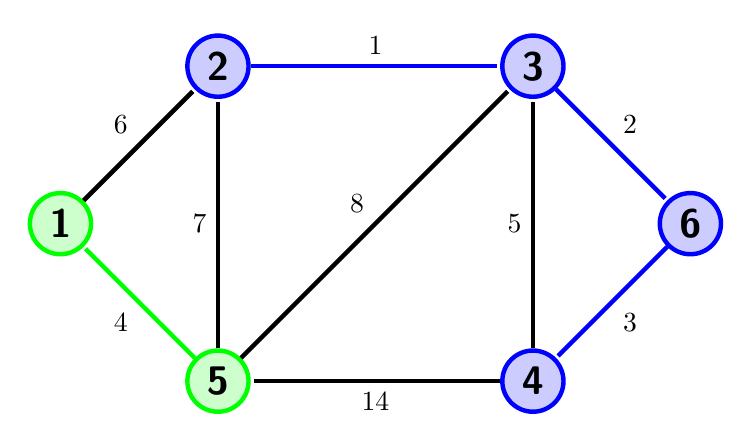
\begin{tikzpicture}[shorten >=1pt, auto, node distance=3cm, ultra thick,
    node_style/.style={circle,draw=green,fill=green!20!,font=\sffamily\Large\bfseries},
    selected_node_style/.style={circle,draw=blue,fill=blue!20!,font=\sffamily\Large\bfseries},
    edge_style/.style={draw=black, ultra thick},
    selected_edge_style/.style={draw=blue, ultra thick},
    selected_edge_style2/.style={draw=green, ultra thick}]

    \node[node_style] (v1) at (-4,0) {1};
    \node[selected_node_style] (v2) at (-2,2) {2};
    \node[selected_node_style] (v3) at (2,2) {3};
    \node[selected_node_style] (v4) at (2,-2) {4};
    \node[node_style] (v5) at (-2,-2) {5};
    \node[selected_node_style] (v6) at (4,0) {6};

    \draw[selected_edge_style]  (v2) edge node{1} (v3);
    \draw[selected_edge_style]  (v3) edge node{2} (v6);
    \draw[selected_edge_style]  (v6) edge node{3} (v4);
    \draw[edge_style]  (v4) edge node{14} (v5);
    \draw[selected_edge_style2]  (v5) edge node{4} (v1);
    \draw[edge_style]  (v1) edge node{6} (v2);
    \draw[edge_style]  (v5) edge node{7} (v2);
    \draw[edge_style]  (v5) edge node{8} (v3);
    \draw[edge_style]  (v4) edge node{5} (v3);
\end{tikzpicture}
\caption{ক্রুসকাল এর অ্যালগরিদম (Kruskal's algorithm)}
\label{fig:kruskal}
\end{figure}

একটি উদাহরণ দেখা যাক। চিত্র ~\ref{fig:kruskal} এ আমরা প্রথমে $2-3$ কে জোড়া দিয়েছি। এরপর $3-6$, $6-4$, $1-5$. ওজনের ঊর্ধ্বক্রমে আসলে আমাদের পরের বাহু হবে $3-4$ কিন্তু এই দুটি নোড একই ট্রি তে আছে সুতরাং আমরা আর এই বাহু জোড়া লাগাব না। এর পরের বাহু হলো $1-2$ এবং এটি দুটি আলাদা ট্রি কে জোড়া লাগায় সুতরাং আমরা এই বাহু নিব এবং ট্রি দুটিকে জোড়া লাগাব। অর্থাৎ যদি ডিসজয়েন্ট সেট ইউনিয়নের ভাষায় বলতে হয়, তাহলে প্রথমে আমরা বাহুগুলোকে মূল্য অনুযায়ী ছোট হতে বড় আকারে সাজাবো। এরপর তাদের একে একে নিবো আর দেখবো এই বাহুর দুই মাথা একই সেটে আছে কি না। থাকলে এই বাহু নিবো না। আর না থাকলে সেই বাহু নেবো আর তাদের দুই মাথার সেটগুলো ইউনিয়ন করে দেব।

এখন প্রশ্ন হলো এই অ্যালগরিদমের টাইম কমপ্লেক্সিটি কত? সহজ, বাহুগুলোকে ওজন অনুযায়ী সর্ট করতে \BigO{m\log{m}} এবং প্রতি বাহুর জন্য আমরা ফাইন্ড (find) করছি বা দুটি সেটকে ইউনিয়ন করছি যাদের কমপ্লেক্সিটি আমরা \BigO{1} ধরে নিতে পারি। সুতরাং \BigO{m\log{m} + m} = \BigO{m\log{m}}.



\begin{figure}[ht!]
\centering
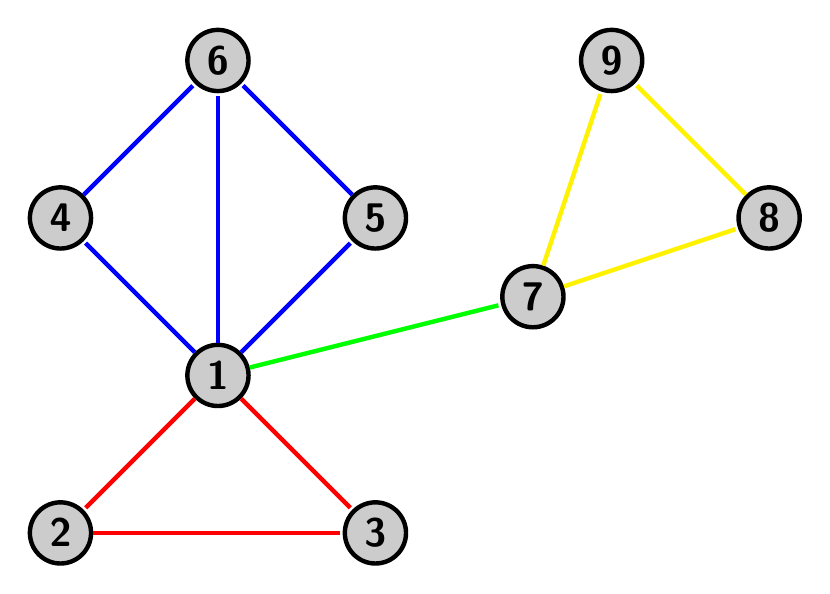
\begin{tikzpicture}[shorten >=1pt, auto, node distance=3cm, ultra thick,
    node_style/.style={circle,draw=black,fill=black!20!,font=\sffamily\Large\bfseries},
    edge_style1/.style={draw=red, ultra thick},
    edge_style2/.style={draw=blue, ultra thick},
    edge_style3/.style={draw=green, ultra thick},
    edge_style4/.style={draw=yellow, ultra thick}]

	\node[node_style] (v1) at (0, 0) {1};
	\node[node_style] (v2) at (-2, -2) {2};
	\node[node_style] (v3) at (2, -2) {3};
	\node[node_style] (v4) at (-2, 2) {4};
	\node[node_style] (v5) at (2, 2) {5};
	\node[node_style] (v6) at (0, 4) {6};
	\node[node_style] (v7) at (4, 1) {7};
	\node[node_style] (v8) at (7, 2) {8};
	\node[node_style] (v9) at (5, 4) {9};

	\draw[edge_style1] (v1) edge node{} (v2);
	\draw[edge_style1] (v1) edge node{} (v3);
	\draw[edge_style1] (v2) edge node{} (v3);
	
	\draw[edge_style2] (v1) edge node{} (v4);
	\draw[edge_style2] (v1) edge node{} (v5);
	\draw[edge_style2] (v1) edge node{} (v6);
	\draw[edge_style2] (v4) edge node{} (v6);
	\draw[edge_style2] (v5) edge node{} (v6);

	\draw[edge_style3] (v1) edge node{} (v7);
	
	\draw[edge_style4] (v7) edge node{} (v8);
	\draw[edge_style4] (v7) edge node{} (v9);
	\draw[edge_style4] (v8) edge node{} (v9);
\end{tikzpicture}
\caption{বাইকানেক্টেড অ্যালগরিদম (Biconnected algorithm)}
\label{fig:bcc}
\end{figure}

তোমরা চিত্র ~\ref{fig:bcc} এ যদি বলতে প্রতিটি বাহু আলাদা আলাদা কম্পোনেন্ট, হ্যাঁ কথা ঠিক কিন্তু এই যে বললাম প্রতিটি কম্পোনেন্টকে আমরা বড় করার চেষ্টা করি, সে জন্য আমাদের BCC হবে চিত্রের মতো।

